\documentclass[conference,a4paper]{APSIPA2026}
\usepackage{cite}
\usepackage{amsmath,amssymb,amsfonts}
\usepackage{graphicx}
\usepackage{textcomp}
\usepackage{xcolor}
\definecolor{figblue}{RGB}{37,84,160}
\definecolor{figred}{RGB}{198,58,45}
\usepackage{booktabs}
\usepackage{array}
\usepackage{multirow}
\usepackage{tikz}
\usetikzlibrary{shapes.geometric,arrows.meta,positioning,calc}
\usepackage{url}
\usepackage{geometry}
\geometry{a4paper, top=19mm, bottom=43mm, right=13mm, left=13mm}
\usepackage{fancyhdr}
\renewcommand{\headrulewidth}{0pt}
\renewcommand{\footrulewidth}{0pt}
\fancypagestyle{firststyle}{%
  \fancyhf{}%
  \fancyhead[C]{2026 Asia Pacific Signal and Information Processing Association Annual Summit and Conference (APSIPA ASC)}%
}
\usepackage[hidelinks]{hyperref}
\graphicspath{{figs/}}
% Float placement: keep every figure and table inside the section that declares
% it. The defaults reserve so much of each column for text that a dense paper
% defers floats across section boundaries.
\renewcommand{\topfraction}{0.92}
\renewcommand{\bottomfraction}{0.85}
\renewcommand{\textfraction}{0.06}
\renewcommand{\floatpagefraction}{0.72}
\setcounter{topnumber}{3}
\setcounter{bottomnumber}{2}
\setcounter{totalnumber}{5}

\begin{document}

\title{An Area-Optimized 8-bit Deep Learning Accelerator\\for GAN Image Generation on GF180MCU}

\author{
\IEEEauthorblockN{William Anthony, I~Made~Medika~Surya~W.M., John~Ruben~Saragi, Mahardhika~Putra~Adipratama,\\
Fairuz~Aquilla~Rahagi, Trio~Adiono, and Infall~Syafalni}
\IEEEauthorblockA{Bandung Institute of Technology, Bandung, Indonesia \\
E-mail: \{13223048, 13222021, 13222049, 13222081, 13222107\}@mahasiswa.itb.ac.id, \\
tadiono@itb.ac.id, infall@ieee.org}
}

\maketitle
\thispagestyle{firststyle}
\pagestyle{empty}

\begin{abstract}
This paper presents an area-optimized 8-bit deep learning accelerator for a small GAN image generator, hardened through a fully open-source flow on the open GF180MCU 180~nm process. The target network is a three-layer multi-layer-perceptron generator trained on MNIST, quantized from FP32 to signed 8-bit integers and mapped onto a structural $4\times4$ processing-element array with a native accumulation depth of $K=256$. Starting from an eleven-macro predecessor, the result buffer is folded from three $256\times8$ SRAM macros used as byte planes into a single $64\times8$ macro addressed along the plane axis, cutting that buffer's area by 77\% and the macro count to nine; the nine macros are then re-arranged onto a $3\times3$ grid and the die squeezed to $1375\times1325~\mu$m. The result is \textbf{24\% less die area and 18\% less power than the eleven-macro design, with more setup margin}, for 11.7\% more compute cycles per image. Antenna closure needed a method the usual placement-density sweep could not supply: the sweep plateaued at a single residual net, but the violating net names identified one specific SRAM macro whose column broadcast was simply placed too far from the array, and swapping it with the small result buffer reached zero violations at two independent densities. The macro signs off with zero DRC, LVS, XOR, and antenna violations at a 40~ns clock across nine STA corners, and is verified bit-exactly against Python golden vectors up to a full 784-pixel image rendered through the routed post-layout netlist.
\end{abstract}

\begin{IEEEkeywords}
Deep learning accelerator, GF180MCU, SRAM macro, area optimization, antenna closure, INT8 quantization, GAN, ASIC, LibreLane, open-source EDA.
\end{IEEEkeywords}

\section{Introduction}
Generative Adversarial Networks can be used as a compact workload for testing neural inference on custom hardware. In this work, the generator is a small MNIST multi-layer perceptron that converts a 64-dimensional latent vector into a $28\times28$ image. The arithmetic is mostly dense matrix multiplication, so the workload can be mapped onto a small array of multiply--accumulate units.

An earlier version of the design used sequential behavioral loops and register memory arrays in Verilog. That version was convenient for checking the algorithm, but not suitable for ASIC implementation: buffers inferred as standard-cell registers make the design too large and difficult to route. The design was therefore restructured into a structural accelerator with a processing-element (PE) array, local SRAM-backed buffers, and a small controller, and hardened as a macro.

That restructured design was signed off with eleven $256\times8$ SRAM macros on a $1600\times1500~\mu$m die. This paper is what happens when the memory of that design is questioned rather than accepted. Three of the eleven macros held the result buffer as byte planes of one 24-bit word, and between them they stored 48 bytes in 768 --- 6.25\% occupancy, on a buffer that the array geometry fixes at sixteen accumulators forever. Folding those three planes onto the address axis of a single $64\times8$ macro recovers 77\% of that area, and removing two macros from the floorplan lets the whole die shrink.

The main contributions are: (1)~a memory-folding transformation that cuts the accelerator's die area by 24\% and its power by 18\% while \emph{improving} setup margin, at a bounded and measured cost in cycles; (2)~an antenna-closure method for when a placement-density sweep plateaus --- reading the violating net names to identify a mis-placed macro, rather than continuing to re-roll the placement --- confirmed by two independent levers reaching zero; (3)~a measured characterization of where the time actually goes, from per-stage cycle counts to an end-to-end estimate over the serial host link; and (4)~a measured justification of INT8 against INT4, INT16, and FP16 on both accuracy and synthesized area.

\section{Related Work}
Most neural network accelerators are built around arrays of multiply-and-accumulate units. A well-known large-scale example is the systolic Tensor Processing Unit \cite{tpu}, and a broad overview of deep learning accelerators for different platforms is given in \cite{survey}. To run a floating-point network on this kind of integer array, the weights and activations are usually quantized with a per-tensor scale, as described by Jacob et al. \cite{jacob}.

Among fabricated accelerators, the reference points span three orders of magnitude in scale. DianNao \cite{diannao} places 496 16-bit fixed-point operators in 3.02~mm$^2$ of 65~nm and reaches 452~GOPS at 485~mW. Eyeriss \cite{eyeriss} spends a 12.25~mm$^2$ 65~nm core on 168 processing elements with a row-stationary dataflow that minimizes data movement, and measures 278~mW at 200~MHz. Closer to our own scale, Wang et al. \cite{wang} present a small reconfigurable PE-array accelerator for an underwater recognition network in 40~nm, at 54.61~GOPS and 96.35~mW. All three are closed-PDK designs on commercial nodes.

The comparison that matters most for the contribution claimed here is against silicon built the same way. OpenSpike \cite{openspike} is a spiking-neural-network accelerator taped out in the open SkyWater 130~nm process using only open-source EDA tools and OpenRAM-generated memory macros, occupying 33.3~mm$^2$ at 40~MHz. Our design shares that open-flow premise but differs in workload and memory strategy: it is an INT8 dense-matrix engine backed by foundry-supplied hard SRAM macros rather than a spiking architecture with generated memory. Section~\ref{sec:perf} places all of these side by side. The workload is a pretrained MLP GAN \cite{goodfellow, ganpretrained}, and the RTL is based on the open DLA Engine project \cite{dlaengine}.

\section{GAN Architecture}\label{sec:overview}

\begin{figure*}[!t]
\centering
\resizebox{\textwidth}{!}{%
\begin{tikzpicture}[x=1mm,y=1mm,
  outerblk/.style={draw=figblue,fill=figblue!4,rounded corners=2.5mm,line width=1pt},
  subblk/.style={draw=figblue!60,fill=white,rounded corners=1.6mm,line width=0.6pt},
  syn/.style={figblue!45,line width=0.3pt},
  flow/.style={-{Stealth[length=1.9mm,width=1.6mm]},figblue,line width=0.9pt},
  ax/.style={-{Stealth[length=1.2mm,width=1.1mm]},black!55,line width=0.4pt},
  fn/.style={figred,line width=1.1pt},
  ttl/.style={font=\scriptsize\bfseries,text=figblue!80!black},
  dim/.style={font=\tiny,text=black!60},
  cell/.style={draw=figblue!75!black,line width=0.35pt,minimum size=3.4mm,inner sep=0pt,font=\tiny}]
% ---- top-level blocks ----
\draw[outerblk] (0,-14) rectangle (19,14);
\draw[outerblk] (26,-15) rectangle (154,19);
\draw[outerblk] (161,-14) rectangle (181,14);
\node[font=\small\bfseries,text=figblue!80!black] at (90,16.1) {MLP GAN Generator};
% ---- fat arrows between top-level blocks ----
\draw[draw=figblue,fill=figblue!15,line width=0.8pt]
  (19.9,1.0) -- (23.2,1.0) -- (23.2,2.1) -- (25.3,0) -- (23.2,-2.1) -- (23.2,-1.0) -- (19.9,-1.0) -- cycle;
\draw[draw=figblue,fill=figblue!15,line width=0.8pt]
  (154.7,1.0) -- (158.0,1.0) -- (158.0,2.1) -- (160.1,0) -- (158.0,-2.1) -- (158.0,-1.0) -- (154.7,-1.0) -- cycle;
\node[dim] at (157.4,3.9) {reshape};
% ---- latent vector, drawn as a vector ----
\node[ttl,align=center] at (9.5,10.6) {Latent\\Vector};
\foreach [count=\i] \val/\sh in {0.8/45, -0.3/14, 1.2/60, -0.7/38}
  \node[cell,fill=figblue!\sh] at (9.5,{4.6-(\i-1)*3.4}) {$\val$};
\node[font=\tiny] at (9.5,-8.15) {$\vdots$};
\node[cell,fill=figblue!28] at (9.5,-10.6) {$0.5$};
\draw[line width=0.5pt,black!75] (7.2,6.6) -- (6.5,6.6) -- (6.5,-12.6) -- (7.2,-12.6);
\draw[line width=0.5pt,black!75] (11.8,6.6) -- (12.5,6.6) -- (12.5,-12.6) -- (11.8,-12.6);
\node[font=\scriptsize] at (9.5,-16.5) {$z\in\mathbb{R}^{64}$};
% ---- dense layers, drawn as neurons ----
\foreach \bx/\lin/\lout/\ltag in {29/64/256/L0, 71/256/256/L2, 113/256/784/L4}{
  \draw[subblk] (\bx,-13) rectangle (\bx+21,13);
  \node[ttl] at (\bx+10.5,10.2) {Dense \lout};
  \node[font=\tiny,text=black!45] at (\bx+2.6,10.9) {\ltag};
  \foreach \ly in {4.2,0,-4.2}
    \foreach \ry in {6.4,3.2,0,-3.2,-6.4}
      \draw[syn] (\bx+5.5,\ly) -- (\bx+15.5,\ry);
  \foreach \ly in {4.2,0,-4.2}
    \node[circle,draw=figblue!80!black,fill=figblue!22,inner sep=0pt,minimum size=3.2mm,line width=0.4pt] at (\bx+5.5,\ly) {};
  \foreach \ry in {6.4,3.2,0,-3.2,-6.4}
    \node[circle,draw=figblue!80!black,fill=figblue!22,inner sep=0pt,minimum size=2.8mm,line width=0.4pt] at (\bx+15.5,\ry) {};
  \node[font=\tiny] at (\bx+5.5,-7.2) {$\vdots$};
  \node[font=\tiny] at (\bx+15.5,-9.3) {$\vdots$};
  \node[dim] at (\bx+5.5,-11.3) {\lin};
  \node[dim] at (\bx+15.5,-11.3) {\lout};
}
% ---- activations, drawn as their functions ----
\foreach \cx/\aname in {60.5/ReLU, 102.5/ReLU, 144.5/Tanh}{
  \draw[subblk] (\cx-6.5,-13) rectangle (\cx+6.5,13);
  \node[ttl] at (\cx,10.2) {\aname};
  \draw[ax] (\cx-4.9,-1.4) -- (\cx+4.9,-1.4);
  \draw[ax] (\cx,-6.3) -- (\cx,3.5);
}
\foreach \cx in {60.5,102.5}{
  \draw[fn] (\cx-4.3,-1.4) -- (\cx,-1.4) -- (\cx+3.4,2.0);
  \node[dim] at (\cx,-8.7) {$\max(0,x)$};
}
\draw[fn,smooth,samples=29,domain=-4.3:4.3] plot ({144.5+\x},{-1.4+3.4*(exp(\x/0.75)-1)/(exp(\x/0.75)+1)});
\node[dim] at (144.5,-8.7) {$\tanh(x)$};
% ---- flow arrows between sub-blocks ----
\foreach \xa in {50.4,67.4,92.4,109.4,134.4}
  \draw[flow] (\xa,0) -- (\xa+3.2,0);
% ---- generated image ----
\node[ttl,align=center] at (171,10.6) {Generated\\Image};
\node[inner sep=0pt] at (171,-2.6) {
\includegraphics[width=12mm,height=12mm]{digit_seed6.jpg}};
\draw[black!60,line width=0.4pt] (165,-8.6) rectangle (177,3.4);
\node[font=\scriptsize] at (171,-16.5) {$28\times28$ grayscale};
\end{tikzpicture}}
\caption{MLP GAN generator: the 64-dimensional latent vector $z$ is expanded through two 256-neuron ReLU hidden layers and a 784-neuron tanh output layer into a $28\times28$ grayscale image (layer tags match Table~\ref{tab:net}).}
\label{fig:gan}
\end{figure*}

The GAN generator architecture, illustrated in Fig.~\ref{fig:gan}, uses a multi-layer perceptron (MLP) model that receives a latent vector of size 64 as the initial input. This input is then projected through two hidden layers, each containing 256 neurons, to form a richer feature representation. Each hidden layer is followed by a ReLU activation function, allowing the model to learn non-linear patterns from the data.

After that, the learned representation is passed to an output layer with 784 neurons, which corresponds to a $28\times28$ pixel image. In the final stage, a tanh activation function is used to limit the output values to a range between $-1$ and $1$, so that the output of the generator can be represented as a grayscale image. Through this process, the generator transforms a random vector into a synthetic image that resembles real data.

Table~\ref{tab:net} lists the three dense layers and shows how many tiles each layer needs on the $4\times4$ array. Because the array produces four output neurons per tile, the layer with 784 outputs needs the most tiles.

\begin{table}[!ht]
\caption{Generator layers and their mapping to the $4\times4$ array.}
\label{tab:net}
\centering
\renewcommand{\arraystretch}{1.08}
\begin{tabular}{@{}lcccc@{}}
\toprule
Layer & Output $\times$ Input & Activation & Tiles & MAC ops \\
\midrule
L0 & $256\times64$  & ReLU & 64  & 16{,}384  \\
L2 & $256\times256$ & ReLU & 64  & 65{,}536  \\
L4 & $784\times256$ & Tanh & 196 & 200{,}704 \\
\midrule
Total & & & 324 & 282{,}624 \\
\bottomrule
\end{tabular}
\end{table}

\section{Hardware Architecture}\label{sec:hw}

The DLA computes a tiled matrix multiplication $C=A\times B$. The array size is $N=4$, and the native accumulation depth is $K=256$, so one transaction accumulates a full 256-term dot product---the inner dimension of the widest generator layers. $K$ is a temporal depth: it sets how many cycles the same 16 PEs accumulate, not the array size. An earlier RTL revision defaulted to $K=4$ and relied on a harness override; since the physical flow synthesizes the bare RTL defaults, the hardened default was widened to $K=256$---a parameter-only change, as the operand SRAMs were already 256 deep. During one transaction, the controller clears the PE accumulators, enables the array for $K$ cycles, and then stores the result block to the C buffer through a writeback path that serializes the sixteen accumulators.

\begin{figure}[!ht]
\centering
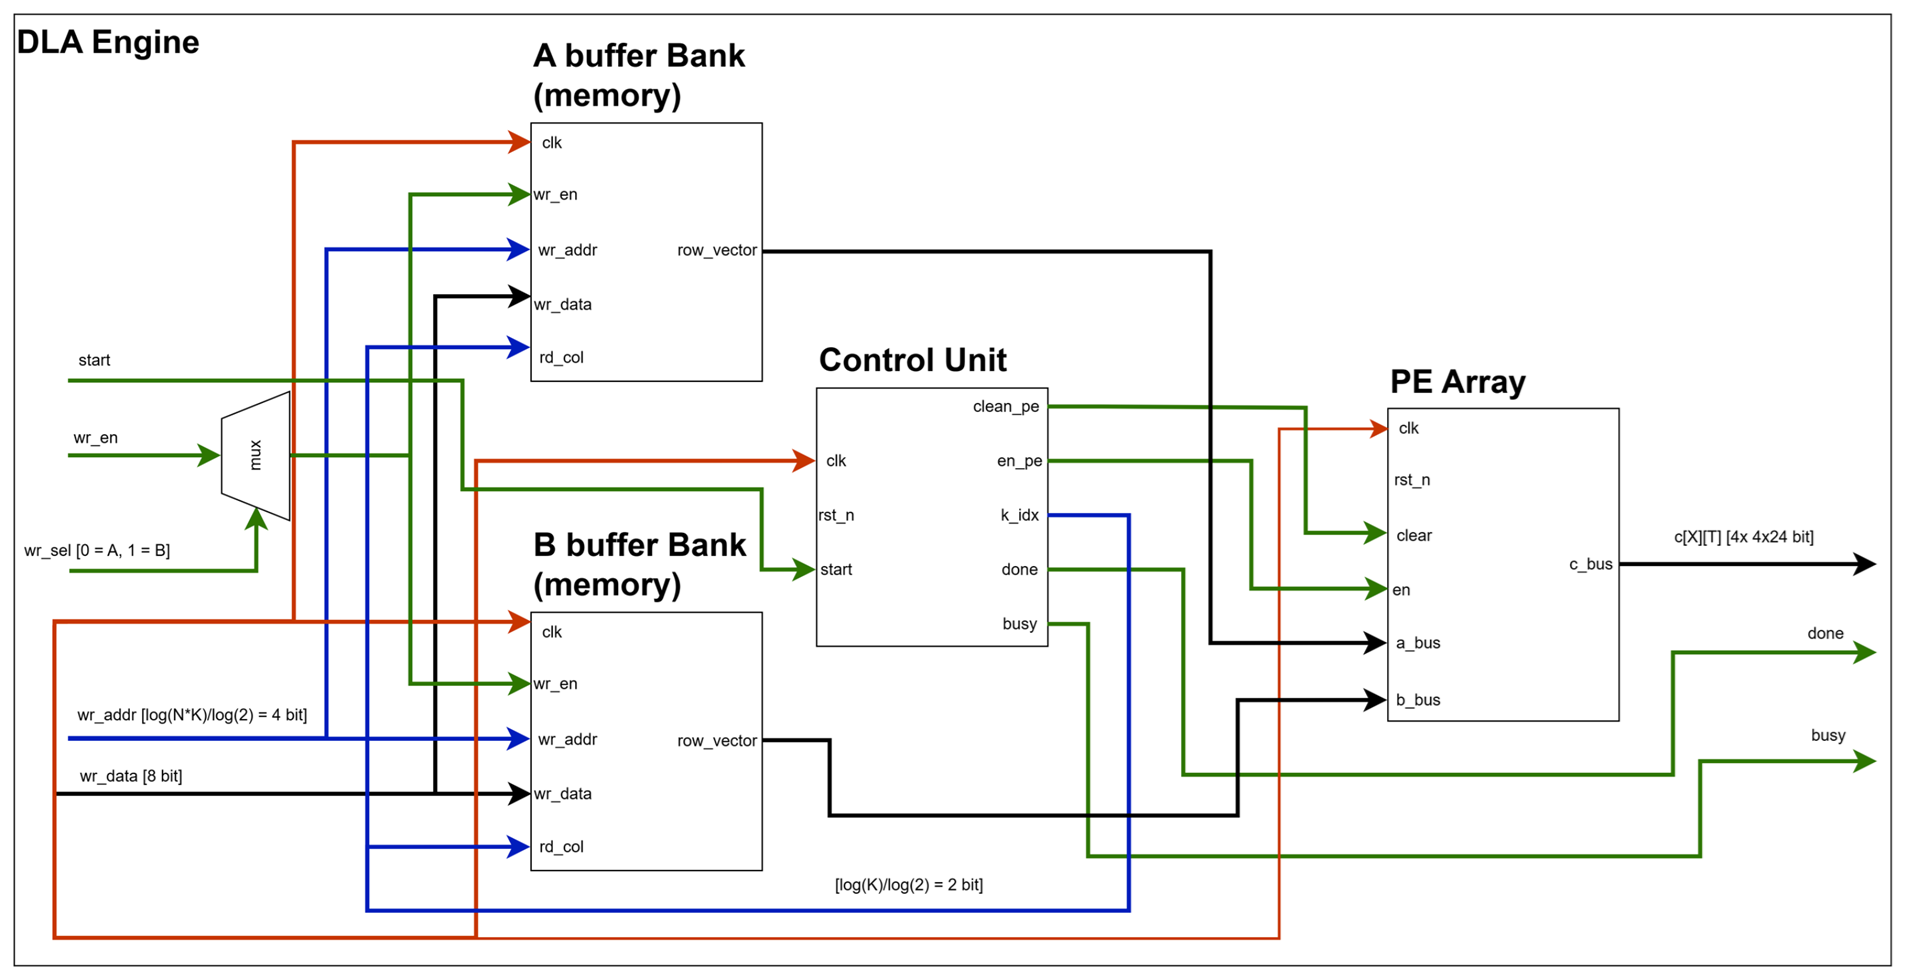
\includegraphics[width=0.66\columnwidth]{Top_level.png}
\caption{DLA engine top level.}
\label{fig:top}
\end{figure}

At the top level, shown in Fig.~\ref{fig:top}, the A buffer provides one row vector to the PE array, and the B buffer provides one column vector. The control unit generates the read index, clear signal, enable signal, done signal, and busy signal. The output bus carries the accumulated C values.

\subsection{Processing Element}

Each processing element (Fig.~\ref{fig:pe}) receives two signed 8-bit inputs. It multiplies them, sign-extends the 16-bit product to 24 bits, and adds it to a local accumulator. The accumulator is cleared at the start of each matrix multiplication. The output of each PE is one dot product.

\begin{figure}[!ht]
\centering
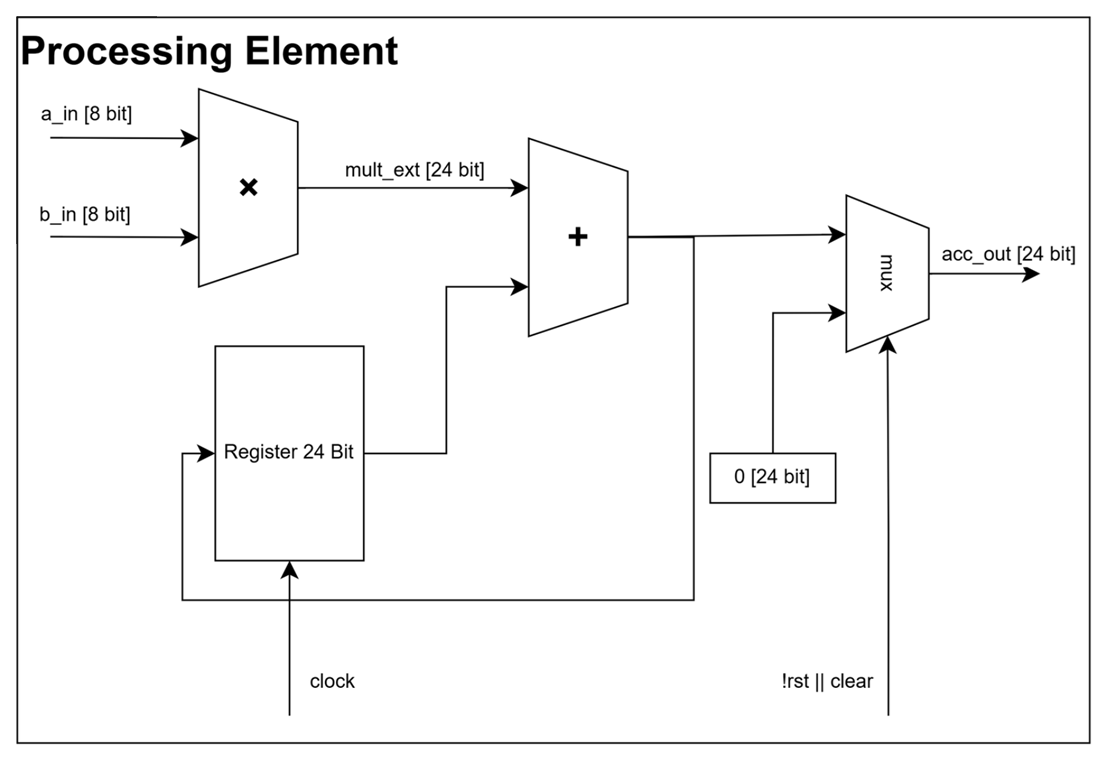
\includegraphics[width=0.62\columnwidth]{PE.png}
\caption{Processing element datapath.}
\label{fig:pe}
\end{figure}

The main computation in one PE follows
\begin{equation}
acc_{out}[n] = acc_{out}[n-1] + a_{in}[n]\,b_{in}[n].
\end{equation}
After $K$ cycles, the accumulator stores one output value of the matrix multiplication tile. A 24-bit accumulator is used so that the sum of 8-bit products has enough range for the selected layer sizes.

\subsection{PE Array}
The PE array (Fig.~\ref{fig:pearray}) instantiates 16 PEs in a $4\times4$ grid. Each row receives one activation lane, and each column receives one weight lane; the operands are broadcast along the rows and columns, and each PE accumulates its result locally (an output-stationary organization), so all 16 PEs operate in parallel and the array produces one $4\times4$ output tile after the accumulation loop finishes.

The $a\_bus$ contains four 8-bit activation values, while the $b\_bus$ contains four 8-bit weight values. The output $c\_bus$ is flattened from 16 accumulator outputs, each with 24 bits.

\begin{figure}[!ht]
\centering
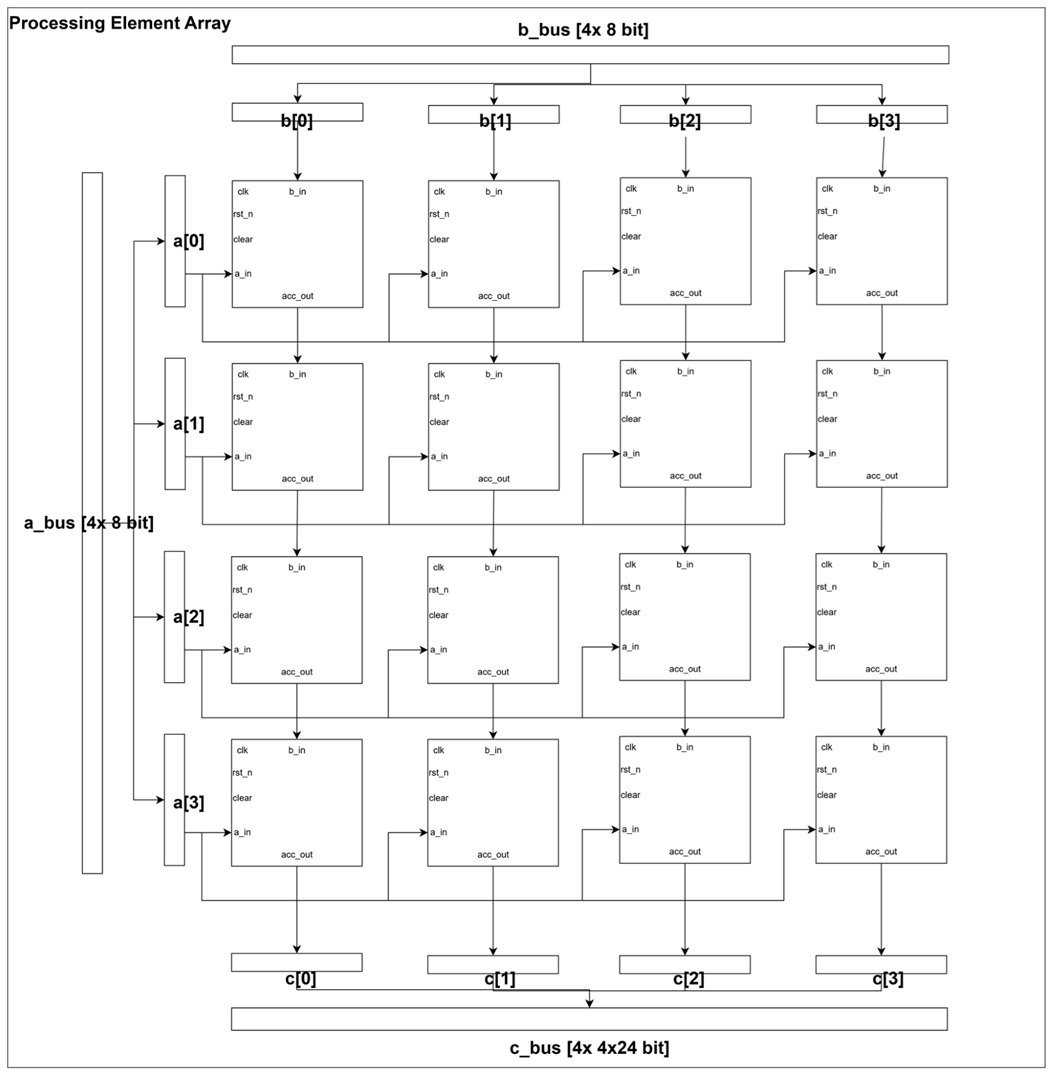
\includegraphics[width=0.70\columnwidth]{PE_Array.png}
\caption{Processing element array.}
\label{fig:pearray}
\end{figure}

\subsection{Controller FSM}
The controller uses four states (Fig.~\ref{fig:fsm}). In IDLE, it waits for START. In CLEAR, it clears all PE accumulators for one cycle. In COMPUTE, it asserts the PE-array enable and increments the A and B buffer addresses until all $K$ terms have been processed. In DONE, it raises DONE and waits for START to return low before going back to IDLE. A separate writeback sequencer then serializes the 16 accumulator values into the C buffer and raises a writeback-done flag.

\begin{figure}[!ht]
\centering
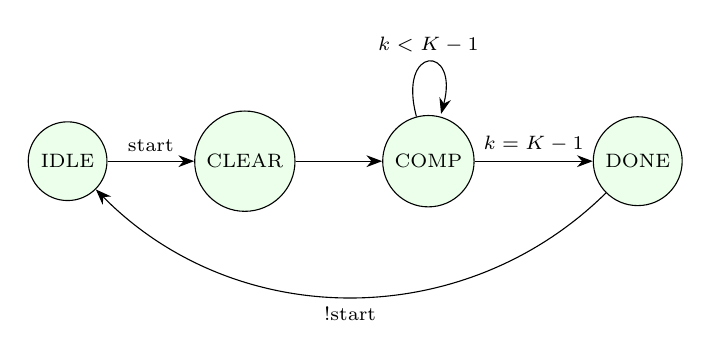
\begin{tikzpicture}[
  font=\scriptsize,>={Stealth[length=2mm]},
  st/.style={draw,circle,minimum size=10mm,fill=green!8}
]
\node[st] (idle) {IDLE};
\node[st,right=11mm of idle] (clear) {CLEAR};
\node[st,right=11mm of clear] (comp) {COMP};
\node[st,right=15mm of comp] (done) {DONE};
\draw[->] (idle) -- node[above]{start} (clear);
\draw[->] (clear) -- (comp);
\path (comp) edge[->,loop above] node{$k<K-1$} (comp);
\draw[->] (comp) -- node[above]{$k=K-1$} (done);
\draw[->] (done) to[bend left=45] node[below]{!start} (idle);
\end{tikzpicture}
\caption{Controller state machine.}
\label{fig:fsm}
\end{figure}

\subsection{SRAM Buffers}
The operand buffers are physical single-port SRAM macros. The A buffer uses four $256\times8$ macros, one per row lane, and the B buffer four more, one per column lane. Eight is a bandwidth floor rather than a capacity choice: the $4\times4$ array consumes four A bytes and four B bytes every compute cycle, and these are 1RW 8-bit parts, so no reduction in depth can reduce the count. Both banks are in any case exactly full at 1{,}024~bytes each.

The C buffer is where the area was. It holds $N\times N=16$ accumulators of 24 bits, which is 48 bytes, and the eleven-macro predecessor stored them as three $256\times8$ macros used as byte planes --- bits [7:0], [15:8] and [23:16] --- sharing one address bus so that a 24-bit word moved in a single access. That spent 203{,}314~$\mu$m$^2$ to store 48 bytes in 768, and no future configuration of this array would ever use the rest: $C$ is $N\times N$ by construction.

This design folds the three planes onto the address axis of one $64\times8$ macro instead, addressing it as
\begin{equation}
\mathit{addr} = \mathit{word}\times 3 + \mathit{plane}, \quad \mathit{word}\in[0,16), \; \mathit{plane}\in[0,3),
\end{equation}
which needs 48 of the 64 available words and costs 45{,}861~$\mu$m$^2$ --- a 77\% reduction, and two fewer macros for the floorplan to route around. Sixty-four is the shallowest depth this SRAM family offers, so this is the floor rather than a tuning point. Total on-chip storage is nine macros and 2{,}112 bytes; the roughly 280~KB of INT8 generator weights are streamed through these tiles from outside rather than stored on chip.

The cost is that 24 bits no longer move in one access. The bank walks the three planes itself: a write holds address and data steady and is acknowledged on the last plane, so writeback takes 48 cycles per transaction instead of 16 --- about $+11.8\%$ against the 256 compute cycles it follows. A read likewise assembles over three plane accesses plus the macro's registered latency, and is valid on the fourth cycle after the read enable rises. That latency is a contract every caller is written against, and Section~\ref{sec:chip} notes where it becomes visible outside the chip.

The SRAM wrapper has a behavioral memory model for simulation and a blackbox branch for synthesis; the power pins are not tied to logic constants in RTL but connected by the physical power delivery network during place and route. The SRAM read has one cycle of latency, so the top level delays the PE enable and completion flags by one cycle to keep data and control aligned, which prevents the PE array from accumulating invalid data after a read request.

\section{Chip-Level Integration}\label{sec:chip}

The hardened accelerator exposes 53 signal bits, but the target shuttle slot provides only 20 general-purpose digital pads next to its 60 analog, 8 supply, clock, and reset pads. Instead of a pin-per-signal mapping, the chip core wraps the accelerator behind a synchronous 4-wire serial bridge (SCLK, MOSI, CS\_N, MISO). The bridge treats SCLK as a data input: all three inputs are double-flop synchronized into the core clock domain and SCLK is edge-detected, deliberately avoiding a second clock domain. A frame is shifted MSB-first while CS\_N is low as a 2-bit command plus a 10-bit address, write frames appending 8 data bits: WRITE\_A and WRITE\_B load the operand buffers, START launches one tile, and READ\_C returns one 24-bit two's-complement result on MISO. Raising CS\_N aborts the frame safely. Three status flags (busy, done, writeback-done) bypass the link and drive pads directly for oscilloscope-visible liveness at bring-up. The chip uses 9 of the slot's 91 pads; the remaining bidir pads are tied off.

One host-visible consequence of the folded C buffer appears here. Because a 24-bit result now assembles over three plane accesses, the bridge must wait longer between presenting a read address and shifting data out: the host must leave roughly nine core clocks after the last address bit rather than four. At the specified SCLK~$\leq$~clk/8 that is a little over one bit period, so in practice the host inserts one idle bit before the read data --- a documented protocol change, and the one place where an internal memory decision reaches the board. The bridge needs one more wait cycle than the on-chip pipeline caller for the same read, because it registers its read enable while the pipeline drives it combinationally.

The padring is the wafer.space GF180MCU project template \cite{padring} for a $2935\times2935~\mu$m workshop slot. One consequence of the template is that the pad supply and the core supply are shorted into a single rail on every pad, so the chip is single-supply by construction. The adopted operating point is therefore 3.3~V for the whole die: the logic and SRAM are 3.3~V parts, and the foundry I/O cells are officially characterized for 3.3~V operation, so every cell operates in a foundry-characterized corner and the I/O levels are directly compatible with a 3.3~V microcontroller host. The predecessor design completed this padring flow with a clean chip-level sign-off, including LVS over 71{,}668 instances; \textbf{that flow has not yet been re-run against the nine-macro macro}, which is the immediate next step and the reason this paper reports macro-level rather than chip-level results.

\section{Software to Hardware Flow}\label{sec:sw}

The system is separated into the hardware core and the verification environment. The hardware core is the DLA engine. It contains the A and B input buffers, the C output buffer, the controller, and the $4\times4$ PE array. This is the part that is hardened and taped out. The verification environment is written in Python and Verilog. It prepares quantized weights, input vectors, and reference outputs, then drives the accelerator through its normal read and write ports---or, at chip level, through the serial protocol exactly as an external host would. On the finished chip, the same role is played by a small microcontroller that streams the tile schedule over the serial link.

\begin{figure}[!ht]
\centering
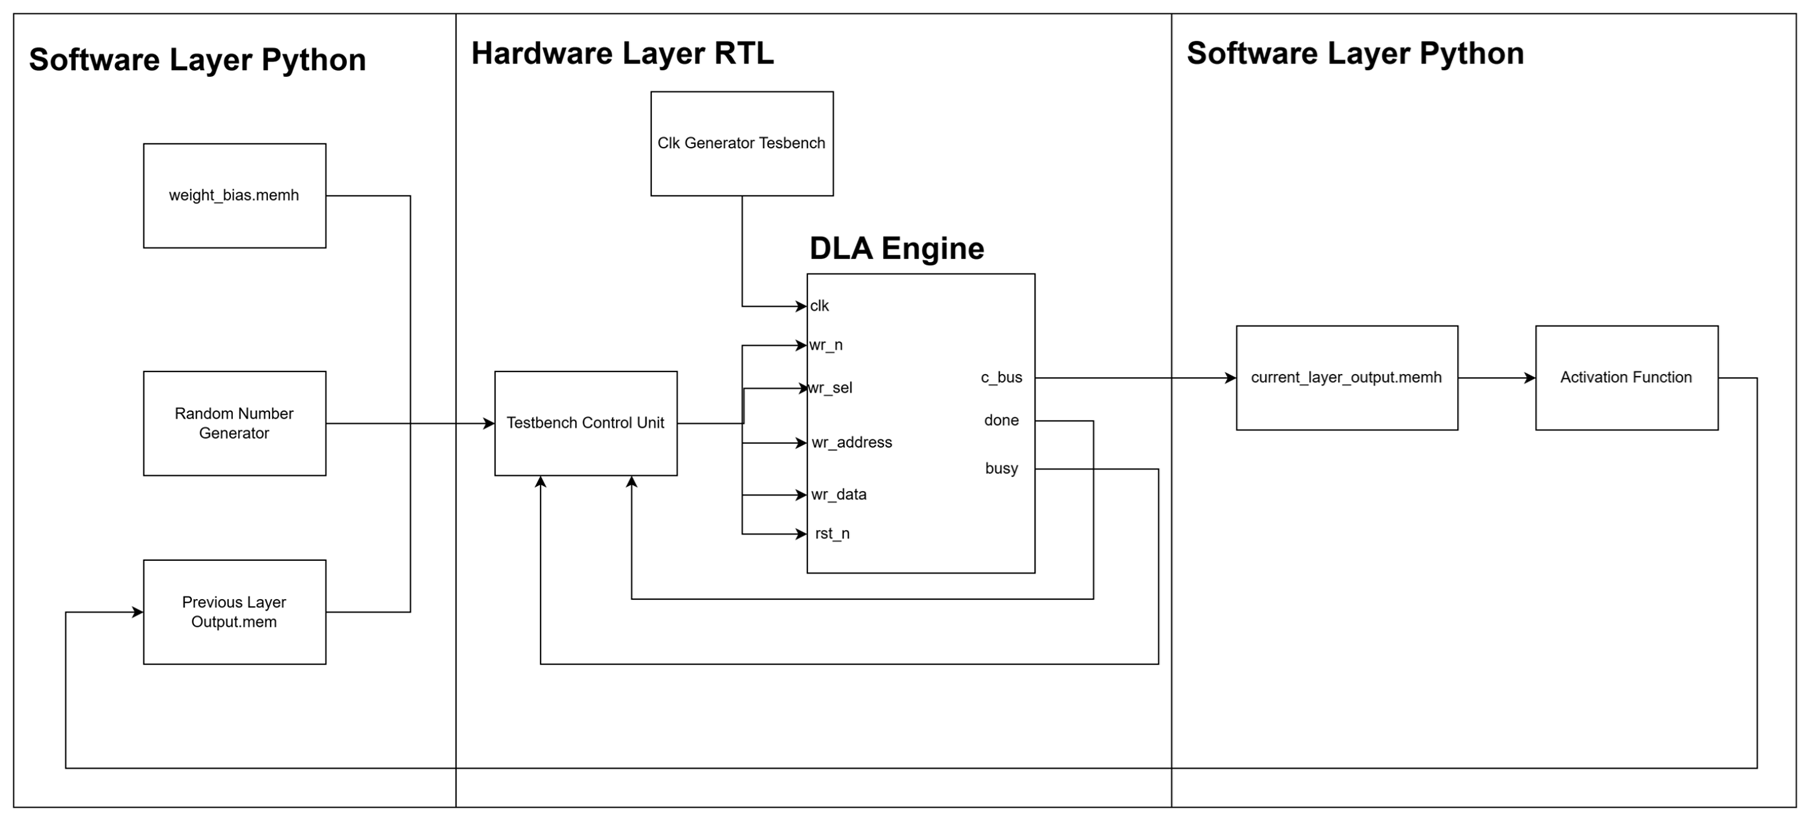
\includegraphics[width=0.55\columnwidth]{Hardware_Software_Integration.png}
\caption{Hardware and software flow.}
\label{fig:hwsoft}
\end{figure}

As shown in Fig.~\ref{fig:hwsoft}, Python prepares the input data and memory contents, then the RTL testbench loads the data into the hardware engine. After the engine finishes, the output is read back and passed to the activation-function stage. This split keeps the accelerator simple, while still allowing the complete GAN pipeline to be checked.

\subsection{Quantization and Requantization}
The original model weights are stored as 32-bit floating-point values. Before they can be used by the integer array, every weight and bias tensor is converted to signed 8-bit values using one scale factor per tensor. The scale comes from the largest absolute value in the tensor, and all scales are saved in a manifest file so the testbench can reuse the same values.

The DLA only returns the integer dot product of one tile. The rest of the math is done around it in integer form, so the hardware result matches the Python reference. For the two hidden layers, the integer result is rescaled, the bias is added, and a ReLU activation is applied before the value is quantized again to 8 bits for the next layer. For the output layer, the result is turned into a fixed-point value, passed through a tanh lookup table, and then mapped to a grayscale pixel. The lookup table is used so that tanh does not have to be computed directly in hardware.

\subsection{Why INT8}\label{sec:format}

\begin{table}[!ht]
\caption{Numeric formats for this generator: accuracy against an exact FP64 render (10 latents, 7{,}840 pixels), and hardware cost. PE area is synthesized on the 3.3~V cells; accumulator width is what 256 accumulated products need.}
\label{tab:format}
\centering
\renewcommand{\arraystretch}{1.08}
\begin{tabular}{@{}lcccrc@{}}
\toprule
 & \multicolumn{2}{c}{Pixel error (gray levels)} & Weights & PE area & Acc. \\
\cmidrule(lr){2-3}
Format & mean & max & (KiB) & ($\mu$m$^2$) & (bits) \\
\midrule
INT4   & 22.26 & 255 & 138 & 6{,}245  & 15 \\
\textbf{INT8}  & \textbf{1.22} & \textbf{72} & \textbf{276} & \textbf{15{,}963} & \textbf{23} \\
INT16  & 0.01  & 1   & 552 & 47{,}037 & 39 \\
FP16   & 0.06  & 5   & 552 & ---      & --- \\
\bottomrule
\end{tabular}
\end{table}
The operand width sets multiplier area, buffer depth, and weight-stream volume at once, so it was chosen by measurement. Each candidate format was applied to the same FP32 checkpoint under this project's quantization scheme and the rendered image compared against an exact FP64 render of the same latent, with error in gray levels of 255; the hardware side is the synthesized area of one PE at each width, the accumulator sized to what $K=256$ requires (Table~\ref{tab:format}).

INT4 is not viable here: a per-tensor scale leaves only seven magnitude steps, and accumulating that coarseness over 256 terms destroys the digit rather than degrading it. INT16 is essentially exact but costs $2.95\times$ the PE area, a 39-bit accumulator, and double the weight traffic --- which, since weight streaming dominates end-to-end latency (Section~\ref{sec:perf}), would double the time per image. FP16 is no more accurate than INT16 while needing the same memory and a different datapath (exponent alignment, normalization, rounding); no PE area is quoted because none was built. INT8 sits at the knee: 1.2 gray levels of average error is invisible in a $28\times28$ digit, the 16-bit product fits the 24-bit accumulator, and the operand width matches the SRAM macro's native word, so the buffers need no packing logic.

\section{Verification}\label{sec:map}

\begin{table}[!ht]
\caption{Verification results.}
\label{tab:verif}
\centering
\renewcommand{\arraystretch}{1.08}
\begin{tabular}{@{}lll@{}}
\toprule
Testbench & Check & Result \\
\midrule
\texttt{d3004\_tb} & one GEMM, single lane & PASS \\
\texttt{d3004n4\_tb} & full $N{=}4$/$K{=}256$ tile, all A/B macros & PASS \\
\texttt{g3005\_tb} & one layer row & PASS \\
\texttt{g300\_pipeline\_tb} & full 784-pixel image & PASS \\
\texttt{chip\_core\_dla\_tb} & pad-level serial protocol & PASS \\
gate-level (unit) & routed 9-macro netlist, $N{=}4$/$K{=}256$ & PASS \\
gate-level (image) & routed 9-macro netlist, 784-pixel image & PASS \\
\bottomrule
\end{tabular}
\end{table}

To verify the GAN RTL result, the generator is mapped onto the DLA as a sequence of tiled dense layers. For each tile, four output neurons are computed at the same time: the four weight rows are written to the A buffer bank, and the shared input vector is written into the B buffer. The DLA then performs the dot products and stores the results in the C buffer. Layer L0 uses the 64-dimensional latent vector as input, and layers L2 and L4 use the 256-dimensional activations of the previous layer; since the array has four output lanes, L0 and L2 each require 64 tiles, while L4 requires 196 tiles. The same datapath is reused for all layers.

Table~\ref{tab:verif} summarizes the stack; all testbenches check against Python golden vectors. The two gate-level runs re-simulate the routed netlist itself --- inserted buffers and roughly 8{,}100 antenna diodes included --- and reproduce the golden results bit-exactly, closing the gap between ``the RTL is correct'' and ``the taped-out netlist is correct.''

Folding the C buffer moved every one of these testbenches, and three of the four things that broke were not obvious in advance. The bank must restart its plane walk when the read address changes and not only when the read enable drops: the unit testbenches hold the enable high across a whole row sweep and merely change the address, and without the restart the planes of consecutive words interleave, assembling a value from two addresses. The serial bridge needs one more wait cycle than the on-chip pipeline caller for the same read, because it registers its read enable while the pipeline drives it combinationally, so the bank sees it a cycle later --- and it must also re-assert that enable in the wait state, since it is a pulse-type output defaulted low each cycle. Finally the testbenches need five clock edges where the RTL callers need four, because a testbench samples the read data in the active region straight after an edge while the RTL callers sample it from a clocked block one region later. Each of these is a consequence of turning one wide access into a sequence of narrow ones, and together they are the real engineering cost of the fold --- larger than the 35 flip-flops it added.

\begin{figure}[!ht]
\centering

\includegraphics[width=0.19\linewidth]{digit_seed6.jpg}\hspace{4mm}

\includegraphics[width=0.19\linewidth]{digit_seed5.jpg}\hspace{4mm}
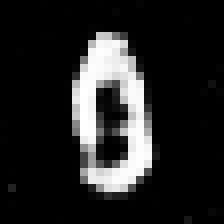
\includegraphics[width=0.19\linewidth]{digit_seed9.jpg}
\caption{Generated digit samples.}
\label{fig:samples}
\end{figure}

Fig.~\ref{fig:samples} shows examples of generated $28\times28$ images. The visual quality is limited by the small generator and by INT8 quantization, but the images are enough to verify that the full software-to-hardware path is running.

\section{Physical Implementation}\label{sec:phys}

The design is implemented with LibreLane \cite{librelane} on the GF180MCU open PDK \cite{gf180pdk}. The accelerator is hardened as a macro whose GDS/LEF/liberty views are what a padring integration consumes; everything reported below is that macro.

\subsection{Single-Supply 3.3~V Library Migration}
The buffer SRAM macro \cite{gf180sram} is a 3.3~V IP, but the open PDK ships only 5~V standard cells, so a first version mixed a 5~V core with 3.3~V SRAMs---workable for layout checks but needing level shifting on silicon. The design was migrated to the third-party \texttt{gf180mcu\_as\_sc\_mcu7t3v3} native-3.3~V library, which ships nine liberty corners and a LibreLane integration, making the die single-supply. Bringing it up surfaced three real bugs in its flow integration (a missing timing-corner variable, a synthesis-exclusion filename mismatch, and non-synthesizable \texttt{\$random} initializers in six sequential-cell models that crashed lint), all fixed at the library source. The 3.3~V cells are much faster than the 5~V ones: the first run at the old 75~ns clock closed with $+44$~ns of setup slack, so the clock was retimed to 40~ns (25~MHz).

\subsection{Hardening the Accelerator Macro}

\begin{table}[!ht]
\caption{Antenna closure on the nine-macro die (40 ns clock, $1400\times1350~\mu$m). All runs are DRC-, LVS-, and timing-clean; only antenna varies. ``Structural'' marks a violator on a \texttt{GEN\_B\_COLS[1]} SRAM output.}
\label{tab:antenna}
\centering
\renewcommand{\arraystretch}{1.08}
\begin{tabular}{@{}llccl@{}}
\toprule
Placement & Density & Nets & Worst & Kind \\
\midrule
grid            & 63 & 1 & $2.18\times$ & structural \\
grid            & 59 & 2 & $1.73\times$ & marginal \\
grid            & 56 & 1 & $1.09\times$ & marginal \\
grid            & 54 & 1 & $1.10\times$ & marginal \\
grid            & 51 & 4 & $1.49\times$ & structural \\
\midrule
\textbf{B/C swap} & \textbf{56} & \textbf{0} & --- & \textbf{sign-off} \\
B/C swap        & 54 & 0 & --- & robustness \\
grid, margin 50 & 56 & 0 & --- & independent \\
B/C swap (re-run) & 56 & 0 & --- & identical DEF \\
\bottomrule
\end{tabular}
\end{table}
A few configuration points were essential. A synthesis define keeps the SRAM as a hard macro---without it, the memory is silently built from flip-flops. The nine macros are registered with their LEF/GDS/liberty views and placed explicitly on a $3\times3$ grid with routing channels. The SRAM power pins only reach Metal3, so the macro power-grid connection had to be made on Metal3 instead of the default higher layers. Routing was allowed up to Metal5, standard-cell padding was added for diode pin access, and antenna diodes are inserted heuristically at placement time with the in-router antenna repair disabled.

Antenna closure is where the nine-macro floorplan behaved differently from its predecessor, and the difference is the methodological result of this paper. In-router antenna repair aborts in this flow because its verification reroute fails pin access on already-placed clock-net diodes, so closure has to come from placement. On the eleven-macro design a one-point perturbation of placement density was enough: it re-rolls which nets route long, and a single nudge cleared the lone marginal net.

Here that lever failed. Table~\ref{tab:antenna} shows five densities across a twelve-point span, and none of them reached zero; they settled into a basin at 54--56 holding one net at about $1.1\times$, with both directions worse. What the sweep produced instead was a diagnosis. The violating net names, which a count alone discards, all pointed at the same place: the outputs of one B-buffer macro, \texttt{GEN\_B\_COLS[1]}, were the $2.18\times$ structural violator at density 63 and returned at $1.49\times$ and $1.18\times$ at density 51, while its eight neighbours never violated once. That macro sat in the corner of the $3\times3$ grid furthest from the PE array, and its column broadcast has to cross the whole die.

That is a placement error wearing an antenna costume. Swapping it into the centre slot and moving the C buffer --- 48 bytes, a short net, never a violator --- out to the corner took the design to \textbf{zero violations}. Two independent checks say this is a fix rather than a lucky re-roll. The same swap is also clean at density 54, where the unswapped floorplan sat at $1.10\times$; and holding the floorplan fixed while instead raising the pre-route diode repair margin from 25 to 50 also reaches zero, from the opposite direction. Two unrelated levers converging says the residual really was those broadcast nets. The swap is the one promoted because it shortens the nets rather than compensating for them, and it costs nothing --- $+16.46$ against $+16.11$~ns of setup slack, and 145 fewer instances.

The general lesson is worth stating plainly: \emph{when a density sweep plateaus, stop sweeping and read the net names.} A violator that survives every density is not a routing lottery, and the sweep's real output is its identity rather than its count.

\begin{figure}[!ht]
\centering
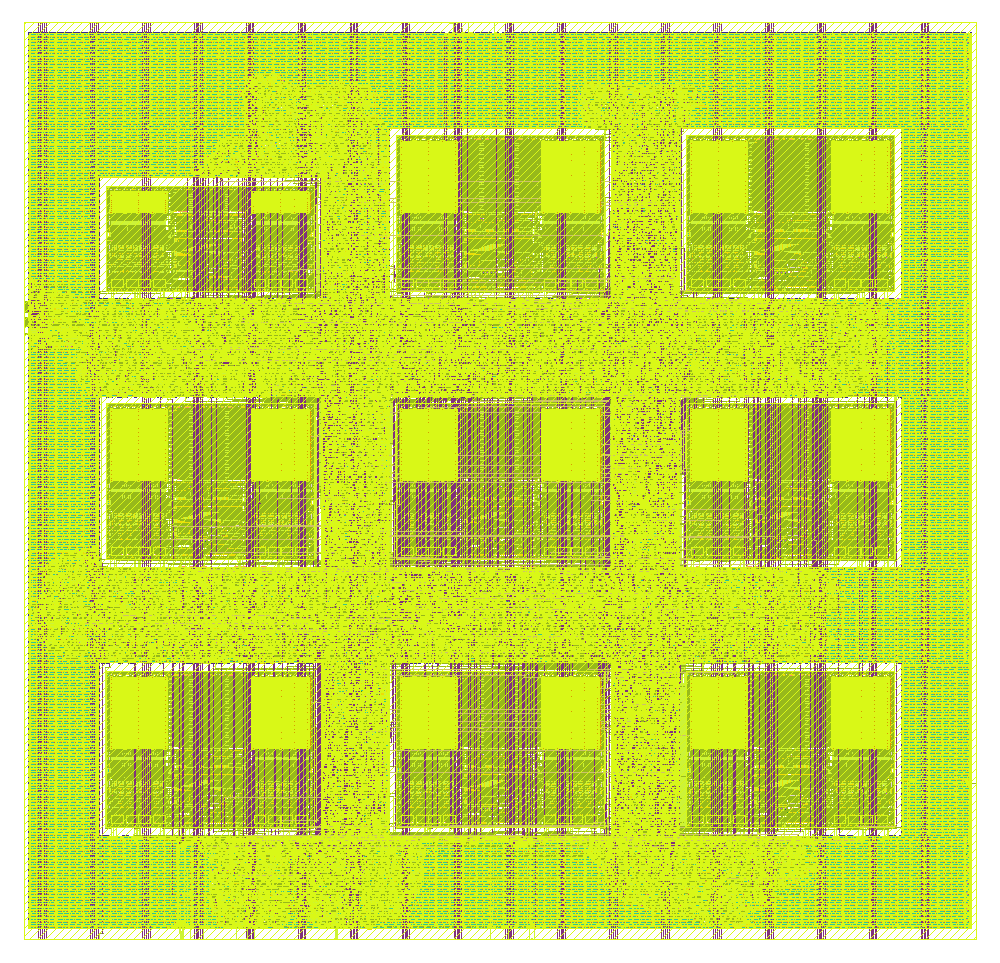
\includegraphics[width=0.72\columnwidth]{Tiny_GDS.png}
\caption{Hardened accelerator macro, $1375\times1325~\mu$m, with the nine SRAM macros on a $3\times3$ grid. The visibly smaller block at the top left is the folded $64\times8$ C buffer, banished to the corner so that the B-buffer macro that kept violating the antenna rule could take the centre slot.}
\label{fig:layout}
\end{figure}

With antenna closed, the die itself was squeezed. Runs at $1400\times1350$, $1375\times1325$ and $1350\times1300~\mu$m keep the swapped topology exactly and scale only the die and the nine macro coordinates, so the channels tighten and nothing is re-rolled. The middle size is the one promoted: shaving 25~$\mu$m off each edge cost 0.22~ns of a 16~ns setup margin and \emph{saved} 2{,}171 instances, which is the relationship seen throughout --- the looser placement is the one carrying more buffering, so tightening pays twice. The smallest size is past the knee: at 56.9\% utilization it leaves two nets barely over at $1.04\times$ and $1.01\times$, and unlike every earlier plateau a density nudge made it worse in both directions ($1.75\times$ at 57, $1.31\times$ at 55). That change of behaviour reads as genuine congestion rather than a re-roll, so the squeeze was stopped there rather than forced.

Fig.~\ref{fig:layout} shows the resulting layout and Table~\ref{tab:signoff} the sign-off. Magic reports zero DRC errors, Netgen zero LVS errors, the GDS cross-check zero XOR differences, and the antenna report zero violating nets and pins. The design meets the 40~ns clock at all nine STA corners (Table~\ref{tab:timing}). The reported nominal power is 133~mW, almost entirely internal power estimated with the flow's default switching activity, and should be read as a conservative tool estimate rather than a measurement.

\subsection{Area and Timing Detail}\label{sec:areatiming}

\begin{table}[!ht]
\caption{Worst slack per PVT corner at the 40~ns clock (worst of the three interconnect models at each point). Zero setup and zero hold violations everywhere.}
\label{tab:timing}
\centering
\renewcommand{\arraystretch}{1.08}
\begin{tabular}{@{}lcccc@{}}
\toprule
 & \multicolumn{2}{c}{This work (9)} & \multicolumn{2}{c}{Predecessor (11)} \\
\cmidrule(lr){2-3}\cmidrule(lr){4-5}
Corner & setup & hold & setup & hold \\
\midrule
SS, 125\,\textdegree C, 3.0 V & $+16.24$ & $+0.360$ & $+15.12$ & $+0.333$ \\
TT, 25\,\textdegree C, 3.3 V  & $+25.15$ & $+0.216$ & $+23.41$ & $+0.260$ \\
FF, $-40$\,\textdegree C, 3.6 V & $+29.19$ & $+0.116$ & $+26.54$ & $+0.150$ \\
\bottomrule
\end{tabular}
\end{table}


\begin{table}[!ht]
\caption{The folded nine-macro design against its eleven-macro predecessor, both antenna-0 and DRC/LVS-clean at 40 ns.}
\label{tab:vs11}
\centering
\renewcommand{\arraystretch}{1.08}
\begin{tabular}{@{}lrrr@{}}
\toprule
 & 11 macros & 9 macros & Change \\
\midrule
Die area (mm$^2$)      & 2.400   & 1.822   & $-24\%$ \\
Core area (mm$^2$)     & 2.326   & 1.761   & $-24\%$ \\
SRAM area ($\mu$m$^2$) & 745,485 & 588,032 & $-21\%$ \\
C buffer ($\mu$m$^2$)  & 203,314 & 45,861  & $-77\%$ \\
Instances              & 93,172  & 79,676  & $-14\%$ \\
Power (mW)             & 162     & 133     & $-18\%$ \\
Wirelength (mm)        & 867     & 812     & $-6\%$ \\
Writeback (cycles)     & 16      & 48      & $+200\%$ \\
Compute per image (ms) & 3.54    & 3.95    & $+11.7\%$ \\
Setup slack, worst (ns) & $+15.12$ & $+16.24$ & better \\
Hold slack, worst (ns)  & $+0.150$ & $+0.116$ & thinner \\
Clock skew, worst (ns)  & 0.65    & 0.44    & $-32\%$ \\
Critical path (ns)      & 24.88   & 23.76   & $-4\%$ \\
\bottomrule
\end{tabular}
\end{table}

\begin{table}[!ht]
\caption{Hardened macro sign-off and core area breakdown.}
\label{tab:signoff}
\centering
\renewcommand{\arraystretch}{1.08}
\begin{tabular}{@{}ll@{}}
\toprule
Metric & Value \\
\midrule
Process & GF180MCU, 180 nm, 3.3 V \\
Standard cells & \texttt{gf180mcu\_as\_sc\_mcu7t3v3} \\
Die area & $1375\times1325~\mu$m \\
Core area (utilization) & 1.761 mm$^2$ (54.8\%) \\
Clock period & 40 ns (25 MHz) \\
Worst setup slack (9 corners) & $+16.24$ ns \\
Worst hold slack (9 corners) & $+0.116$ ns \\
Magic DRC / Netgen LVS / XOR & 0 / 0 / 0 \\
Antenna & 0 nets, 0 pins \\
Power (nominal, tool estimate) & 133 mW \\
Routed wirelength & 812 mm \\
Total instances & 79,676 \\
\midrule
\multicolumn{2}{@{}l}{\emph{Core area breakdown (cells / $\mu$m$^2$)}} \\
SRAM macros ($8\times256$, $1\times64$) & 9 / 588,032 (33.4\%) \\
Combinational logic & 9,936 / 242,313 (13.8\%) \\
Well taps & 8,763 / 38,473 (2.2\%) \\
Antenna diodes & 8,145 / 35,760 (2.0\%) \\
Sequential cells & 441 / 35,292 (2.0\%) \\
Buffers, inverters, ties & 1,987 / 25,971 (1.5\%) \\
Fill and decap & 50,395 / 686,907 (39.0\%) \\
\bottomrule
\end{tabular}
\end{table}
The lower panel of Table~\ref{tab:signoff} resolves the core area, and it shows both what the fold achieved and what it did not. The nine macros take 0.588~mm$^2$ against the predecessor's 0.745~mm$^2$, a 21\% cut of total SRAM area from a 77\% cut of one buffer. The floorplan remains memory-dominated --- macros are still 33\% of the core against 21\% for all placed standard cells --- because the eight A and B macros are a bandwidth floor rather than a capacity choice and cannot be folded the same way. The arithmetic itself is a minority of the logic: 0.242~mm$^2$ of combinational cells against 0.074~mm$^2$ of well taps and the 8{,}145 antenna diodes inserted at placement. Sequential area rises slightly, from 406 to 441 flip-flops, which is the plane-walking state machine the folded buffer needs --- 35 flip-flops bought 157{,}453~$\mu$m$^2$ of macro.

Timing is signed off at nine corners --- three PVT points crossed with minimum, nominal, and maximum interconnect --- and Table~\ref{tab:timing} gives the worst interconnect model at each PVT point. Setup is governed by the slow corner and hold by the fast one, both with margin. Notably the area reduction \emph{improved} setup: $+16.24$~ns against the eleven-macro design's $+15.12$~ns, because a smaller die shortens the same nets that the critical path runs on. That path goes from an SRAM read through the operand multiplexing into the MAC and back to the accumulator register --- making A and B SRAM rather than registers is what puts a macro read on a combinational path, and at the slow corner the macro's own clock-to-output is 12.6--15.0~ns of it, depending on load. The remaining slack puts the true critical path at 23.76~ns, so the macro would close near 42~MHz; the 25~MHz operating point is a deliberate $1.7\times$ guard band on a first tapeout in an unfamiliar library. Hold slack is the thinnest number in the sign-off at $+0.116$~ns, slightly thinner than the predecessor's $+0.150$~ns, and is set by clock-tree skew (0.44~ns) rather than by the period. It is what to watch if a floorplan change moves the clock tree.


Table~\ref{tab:vs11} collects the whole comparison. The fold pays on every physical axis at once --- 24\% of the die, 21\% of the SRAM area, 14\% of the instances, 18\% of the power --- and improves setup margin rather than trading against it. What it costs is cycles, and only in one place: writeback grows from 16 to 48 cycles per transaction, which is 11.7\% more compute time per image and, as Section~\ref{sec:perf} shows, 0.04\% of end-to-end latency once the host link is accounted for.

\clearpage
\section{Performance}\label{sec:perf}

\subsection{Latency Breakdown}

\begin{table}[!ht]
\caption{End-to-end latency for one $28\times28$ image, at a 25~MHz core clock and the nominal SCLK of 3.125~MHz (clk/8). On-chip cycles are measured from the full-image simulation of this design; link times are computed from the protocol's frame lengths at that rate, the frame sequence itself having been verified at the pads.}
\label{tab:latency}
\centering
\renewcommand{\arraystretch}{1.08}
\begin{tabular}{@{}lrrr@{}}
\toprule
Stage & Frames & Time (ms) & Share \\
\midrule
Weight tiles $\rightarrow$ A buffer & 331{,}776 & 2{,}123.4 & 98.85\% \\
Input vector $\rightarrow$ B buffer & 768       & 4.9       & 0.23\% \\
START commands                      & 324       & 1.2       & 0.06\% \\
Compute + writeback (on chip)       & 324 tiles & 4.0       & 0.18\% \\
Result readback from C              & 1{,}296   & 15.3      & 0.71\% \\
\midrule
Total                               &           & 2{,}149   & 0.47 img/s \\
\bottomrule
\end{tabular}
\end{table}
The array performs 16 MAC operations per cycle, a peak of 0.8~GOPS at 25~MHz; quoting only that would be misleading, so this section separates what the array costs from what feeding it costs. The on-chip cycle counts are measured by instrumenting the full-image RTL simulation per controller state, and the link times follow from the frame lengths of Section~\ref{sec:chip}.

Per tile the engine is busy 305 cycles: one CLEAR, 256 accumulation cycles, and 48 writeback cycles walking the sixteen accumulators through the folded buffer's three byte planes. Over 324 tiles that is 98{,}820 cycles, or 3.95~ms at 40~ns --- the ``pure compute'' figure, and 17.9\% of peak, against 3.54~ms and 20.0\% for the eleven-macro design. The 11.7\% penalty is exactly the writeback growth and nothing else; the accumulation itself is untouched. The shortfall is structural, not a scheduling defect: the generator evaluates a matrix--\emph{vector} product, so only the four PEs of B's first column produce useful neurons while the other twelve recompute against unused columns; batching four latents would recover most of it with no hardware change. Feeding the array costs far more. Each tile needs its four weight rows written across the full $K=256$ depth, 1{,}024 bytes, and every byte is one 20-bit frame. The bridge synchronizes and edge-detects SCLK, so the link is specified at SCLK~$\leq$~clk/8 --- 3.125~MHz, 320~ns per bit, 6.4~$\mu$s per byte (Table~\ref{tab:latency}).

End-to-end latency is therefore \textbf{2.149~s per image} (0.47 images/s) against 4.0~ms of arithmetic: the serial link is 99.8\% of it and weight streaming alone 98.8\%, giving an effective 263~kOPS. This is where the area trade is settled. The folded buffer costs 0.41~ms of extra compute and another 0.41~ms of slower result reads, together 0.04\% of the time an image takes; it buys 24\% of the die. At this operating point the exchange is close to free, and it would remain favourable even if the link were made an order of magnitude faster. The bottleneck is not link width alone but the workload's zero weight reuse --- a matrix--vector product touches every weight once, so 1.01 bytes must cross the interface per MAC however that interface is built. Even an idealized parallel port taking one byte per core clock leaves weight loading at 331{,}776 of 440{,}903 cycles, still 75\%. Some traffic is avoidable: the schedule writes the full 256-deep A tile even for L0, whose inputs are 64 wide, so a host that pre-zeroes the tail sends 282{,}624 bytes and finishes in 1.83~s. This is the trade the pad budget forced --- 20 pads and 2.1~KB of SRAM against 280~KB of weights --- and it is where future work belongs: a burst write that sends the address once would remove 12 of every 20 bits, and a wider host bus scales further.

\subsection{Comparison}

\begin{table}[!ht]
\caption{Comparison with representative deep learning accelerators. Throughput is peak ($2\times$ MACs $\times$ frequency); efficiency is peak throughput over reported power. Our power is a tool estimate, not a measurement.}
\label{tab:compare}
\centering
\small
\renewcommand{\arraystretch}{1.12}
\begin{tabular}{@{}lccrrc@{}}
\toprule
 & Tech. & Area & Peak & Eff. & Open \\
Design & (nm) & (mm$^2$) & (GOPS) & (GOPS/W) & flow \\
\midrule
DianNao \cite{diannao}   & 65  & 3.02  & 452   & 932 & No \\
Eyeriss \cite{eyeriss}   & 65  & 12.25 & 67.2  & 242 & No \\
Wang \emph{et al.} \cite{wang} & 40 & 11.97 & 54.61 & 567 & No \\
OpenSpike \cite{openspike} & 130 & 33.3 & ---   & 56.8 & Yes \\
\textbf{This work}       & 180 & \textbf{1.76} & 0.8 & 6.0 & \textbf{Yes} \\
\bottomrule
\end{tabular}
\end{table}
Table~\ref{tab:compare} places this work against three fabricated accelerators on commercial nodes \cite{diannao, eyeriss, wang} and one built, like ours, entirely with open tools on an open PDK \cite{openspike}. Throughput and efficiency are peak figures ($2\times$ MACs $\times$ frequency) so that very different scales compare on one basis.


The gap should be read plainly: two to three orders of magnitude below the commercial-node parts in peak throughput and about two in efficiency. Almost none of it is architectural. A $4\times4$ array at 25~MHz has $31\times$ fewer multipliers than Eyeriss at $8\times$ the clock, which accounts for the throughput difference by itself, and the efficiency difference is what 180~nm at 3.3~V costs against 65~nm and below. The comparison that isolates the contribution is OpenSpike, the other open-PDK, open-flow tapeout: at a similar scale and clock this design occupies 1.76~mm$^2$ against 33.3~mm$^2$ and uses foundry-supplied hard SRAM macros rather than generated memory. What this work offers is not performance but reproducibility and density --- every step from the quantization scripts to the final GDS runs on public tools and a public PDK, and the memory-folding transformation is applicable to any accumulator buffer whose depth is fixed by array geometry rather than by the workload.

\section{Discussion}\label{sec:disc}
Two results here generalize beyond this chip. The first is that buffer depth and buffer \emph{shape} are separable. The C buffer's problem was never capacity --- 48 bytes in a 768-byte allocation --- but that a byte-plane organization spends one macro per byte of word width, and macro count, not macro occupancy, is what the floorplan pays for. Folding planes onto the address axis converts a width cost into a latency cost, and that exchange is attractive whenever the buffer sits off the critical path, as an accumulator writeback does. The transformation is not specific to this design: any accumulator buffer whose depth is fixed by array geometry rather than by the workload is over-provisioned in the same way.

The second is about the antenna methodology. A density sweep is a re-roll, not an optimization, and its output should be read as evidence rather than as a score. Here five densities produced no zero but did produce a consistent name, and acting on the name closed the problem in one run. The cost of the plateau was five runs of several hours each; reading the net names after the second would have saved most of that.

The remaining performance limits are unchanged from the predecessor. A tile engine with no weight reuse is interface-bound at any interface width, and the 2.1~KB of on-chip SRAM against 280~KB of weights is the pad budget's consequence. The levers that would matter are, in order: batching several latents through the array's unused columns, which costs no hardware; a burst write command amortizing the address over many bytes; and a wider host bus. None requires the datapath to change.

The implementation also shows a trade-off between timing and antenna closure: floorplans that shortened the SRAM-to-MAC critical path consistently increased the antenna count, and the priority here was a clean physical sign-off rather than the fastest possible clock. The earlier voltage-domain concern was resolved structurally---the padring shorts the pad and core supplies, so the single-supply 3.3~V operating point removes the level-shifting problem entirely, at the cost of 3.3~V (rather than 5~V) I/O levels, which matches the intended microcontroller host anyway. A true dual-rail variant was evaluated and deferred because the only available dual-voltage pad library is not yet silicon-ready. A bring-up plan for the returned silicon is prepared: current-limited power-on, status-pin checks, replay of the unit-test golden vectors over the serial link from a bit-banging 3.3~V microcontroller, and finally a full streamed digit render.

\section{Conclusion}\label{sec:concl}
This work takes a signed-off INT8 GAN-generator accelerator on GF180MCU and makes it 24\% smaller by questioning its memory rather than its logic. Folding the result buffer's three byte planes onto the address axis of a single $64\times8$ macro cuts that buffer by 77\%, removes two macros from the floorplan, and allows a $3\times3$ arrangement on a $1375\times1325~\mu$m die that also draws 18\% less power and closes with \emph{more} setup margin, for 11.7\% more compute cycles --- 0.04\% of end-to-end latency in practice. Antenna closure, which a placement-density sweep could not deliver, came instead from reading the violating net names and moving the one macro they named, confirmed by two independent levers reaching zero. The macro passes DRC, LVS, XOR, and antenna checks cleanly at 40~ns across nine corners on a single 3.3~V supply, and is verified bit-exactly up to a full-image render on the routed netlist. The immediate remaining work is to re-run the padring integration against this macro, and then silicon bring-up.

\section*{Acknowledgment}
The authors thank the open-source EDA community, the GlobalFoundries open PDK program for GF180MCU and the SRAM macro, and the wafer.space chipathon program for the padring template and the shuttle slot targeted by this work.

\begin{thebibliography}{15}
\bibitem{tpu} N. P. Jouppi \emph{et al.}, ``In-datacenter performance analysis of a tensor processing unit,'' in \emph{Proc. ISCA}, 2017.
\bibitem{survey} C. Silvano \emph{et al.}, ``A survey on deep learning hardware accelerators for heterogeneous HPC platforms,'' \emph{ACM Computing Surveys}, 2025.
\bibitem{diannao} T. Chen, Z. Du, N. Sun, J. Wang, C. Wu, Y. Chen, and O. Temam, ``DianNao: a small-footprint high-throughput accelerator for ubiquitous machine-learning,'' in \emph{Proc. ASPLOS}, 2014, pp.~269--284.
\bibitem{eyeriss} Y.-H. Chen, T. Krishna, J. S. Emer, and V. Sze, ``Eyeriss: an energy-efficient reconfigurable accelerator for deep convolutional neural networks,'' \emph{IEEE J. Solid-State Circuits}, vol.~52, no.~1, pp.~127--138, Jan. 2017.
\bibitem{openspike} F. Modaresi, M. Guthaus, and J. K. Eshraghian, ``OpenSpike: an OpenRAM SNN accelerator,'' in \emph{Proc. IEEE ISCAS}, 2023.
\bibitem{jacob} B. Jacob, S. Kligys, B. Chen, M. Zhu, M. Tang, A. Howard, H. Adam, and D. Kalenichenko, ``Quantization and training of neural networks for efficient integer-arithmetic-only inference,'' in \emph{Proc. IEEE/CVF CVPR}, 2018.
\bibitem{wang} C. C. Wang, S. H. Luo, H. C. Wu, R. G. B. Sangalang, C. P. Jou, and H. Hsia, ``A 54.61 GOPS 96.35 mW digital logic accelerator for underwater object recognition DNN using 40 nm CMOS process,'' in \emph{Proc. IEEE 6th Int. Conf. AI Circuits and Systems (AICAS)}, 2024.
\bibitem{goodfellow} I. Goodfellow, J. Pouget-Abadie, M. Mirza, B. Xu, D. Warde-Farley, S. Ozair, A. Courville, and Y. Bengio, ``Generative adversarial nets,'' in \emph{Proc. NeurIPS}, 2014.
\bibitem{ganpretrained} C. Singh, ``GAN/VAE pretrained PyTorch models,'' \url{https://github.com/csinva/gan-vae-pretrained-pytorch}.
\bibitem{dlaengine} ``DLA Engine,'' GitHub, \url{https://github.com/wlmoi/DLA_Engine}.
\bibitem{padring} wafer.space, ``GF180MCU project template,'' \url{https://github.com/wafer-space/gf180mcu-project-template}.
\bibitem{librelane} The LibreLane project, ``LibreLane: an open-source RTL-to-GDSII flow,'' \url{https://github.com/librelane/librelane}.
\bibitem{gf180pdk} GlobalFoundries and Google, ``GF180MCU open-source PDK,'' \url{https://github.com/google/gf180mcu-pdk}.
\bibitem{gf180sram} R. T. Edwards, ``GF180MCU OCD IP SRAM macros,'' \url{https://github.com/RTimothyEdwards/gf180mcu_ocd_ip_sram}.
\end{thebibliography}

\end{document}